%this will contains the latex report
\documentclass{article}
\usepackage[utf8]{inputenc}
\usepackage{amsmath}
\usepackage{amsfonts}
\usepackage{xcolor}
\usepackage[allcolors=blue]{hyperref}
\usepackage{cleveref}
\usepackage{dirtytalk}
\usepackage{graphicx}
\usepackage{float} %fixe image position
\usepackage[ruled,vlined]{algorithm2e}
% hyperlink
\usepackage{hyperref}
\hypersetup{
    colorlinks=true,
    linkcolor=blue,
    filecolor=magenta,
    urlcolor=cyan,
    }
\title{\Large Report for AMIES challenge, Wasserstein-blind group:\ Automatic data quality assessment}

\author{Abaach Mariem, Boussaa Mehdi, Hawat Diala}
\usepackage{fancyhdr}
%\pagestyle{fancy}
%\makeatletter
%\let\runauthor\@author
%\let\runtitle\@title
%\makeatother


\date{}

\newcommand\dhawat[1]{\textcolor{red}{DH: #1}}
\newcommand\mabaach[1]{\textcolor{magenta}{MA: #1}}
\newcommand\mboussaa[1]{\textcolor{blue}{MB: #1}}


\begin{document}
\maketitle

\begin{abstract}
    Data is what guides today's decision making process, everyone relies on it, it is at the center of modern institutions, but according to the saying : GIGO (Garbage In Garbage Out), bad data may have detrimental consequences on the company that used it.  It is then of crucial order that the data be of best quality possible, however, the process of cleaning the data usually relies on deterministic rules, which makes it hard, tedious and time consuming. Thus AMIES along with the company Foyer proposed a challenge about the automation of the process. This problem required us to first assess what we meant by ``good data quality'' which led to a definition of data quality and to proposed algorithms that need as little as possible of human intervention.
\end{abstract}
\tableofcontents
\section{Intoduction} % (fold)
\label{sec:Intoduction}
With any form of decision making, the quality of the decision is only as good as the data analysed, and so there is a need to ensure that the highest quality data is available for analysis. While having good levels of data quality improves analysis accuracy, having bad data quality can have a serious impact on the enterprise.
Poor data quality has a substantial impact, such as financial loss.  \href{https://www.ibm.com/blogs/journey-to-ai/}{IBM} estimate the loss of 3.1 trillion dollars annually  in the USA due to poor data quality which is twice \href{https://data.worldbank.org/indicator/NY.GDP.MKTP.CD}{Canada’s GDP} in the very same year. Productivity loss, \href{https://www.forrester.com/report/Build-Trusted-Data-With-Data-Quality/RES83344}{Forrester} came up with a study that 40\% of data scientists spend 1/3 of their time validating and fixing data quality issues. All of that lead to a low trust in data.
Traditional data quality control methods are based on users’ experience or previously established business rules, and this
limits performance in addition to being a very time consuming process and low accuracy.

The main purpose of this research is to examine the possible use of probability and machine learning techniques to improve indicators
of data quality in a given dataset, with no domain specific knowledge.
There was no particular regard to the domain of the dataset chosen, the main criteria for choice was the concept that bad data or outlier are rare data objects, \textit{i.e.} , those objects with rare combinations of feature and values, compared to the majority of objects.
We built a package of Python algorithms to detect bad data present in any type of table of data. Those algorithms are gathered in a Python class easy to use, and provided with detailed documentations, facilitating the comprehension and opening the door for further development of this class. The class contains test for many type of outlier (bad data) that could be found in a table of data such as: detection of repetition row, break of uniqueness rule, search for extreme values for columns with density distribution, non significant rows and columns, detection of spelling errors, and typographical error, outlier detection over rows, in each column and in each category of the columns with discrete distribution, detection of logical error between correlated columns.

This short survey is a report on the problem of data quality proposed by the company \href{ https://www.foyer.lu/en/homepage}{Foyer} during the challenge \href{https://challenge-maths.sciencesconf.org/}{\textit{mathematiques et entreprises}} organized by AMIES,  SFdS, SMF and SMAI.
In section \ref{sec:Data quality} what data quality is and different metrics used to asses it, and the difficulty arising while trying to find bad data, or to estimate the quality of the table in general. Then in section \ref{sec:Starategy used to detect bad data} we detail our strategy used to deal with bad data. This section present theoretical mathematical concept behind the tests present in our Python package. In section \ref{sec:Algorithm}, we present some of the principal code used in our package described in section ref{sec:Starategy used to detect bad data}. In section \ref{sec:Experiments} we present the results of the test of our code on the table of data provides by the company \href{ https://www.foyer.lu/en/homepage}{Foyer} to test the efficiency of our methods. Finally, in section \ref{sec:Discussions}, we present the limitations of our algorithm and we propose solutions to overcome this limitations, and develope further the package.

% sectionIntoduction (end)

\section{Data quality} % (fold)
\label{sec:Data quality}
Starting from the basic problem, what can we consider as being good data?
In an idyllic world, when we proceed to do data collection, we target data with no duplicated rows, no missing values, no typos or illogical errors, in a sense, no alteration of the picture that we are trying to capture from the real world.
More specifically, in classification issues, the target is homogeneous data where all classes are equally represented.
But of course, this is not what we obtain.
Hence, we refer to data quality as a quantification of the difference between our ideal expectations and the available result and we project these differences to several axes.
The trade-off is to consider two basic axes.
First, the \textit{extension} of the data focusing our attention on data values and second the \textit{intension} of the data representing the logical view of the database \cite{amazon}.
The two are interconnected.
The latter is harder to measure, but highly influences the applicability of the extension's range of attributes.
Regarding the extension and the intension axes, the quality of data is subject to different metrics.
The first and most obvious one is \textit{redundancy} which refers to duplicated instances i.e., repeated rows or columns.
Second \textit{completeness} i.e., the comprehensiveness or wholeness of the data, measured by the presence of missing data.
However, completeness should be considered in the right context.
For example, in the schema of product category, the absence of a value for an attribute \texttt{shoe\_size} is not relevant for a product in the category \texttt{notebooks} \cite{amazon}.
Thus measuring completeness is only relevant when the attribute is applicable.
\textit{Consistency} as the degree to which a set of semantic rules are violated.
It define the range of admissible values within a column i.e., a specific data type, an interval for numerical columns, or a set of values for categorical ones.
It represents the logical inter-connectivity and interrelationship of the columns.
Finally, the \textit{Accuracy}, which refers to whether the values stored are the correct values.
More precisely, data values must be the right values and must be represented in a consistent and unambiguous form.
We can identify two characteristics of accuracy.
The form and the content.
The form eliminates ambiguities about the content.
For example, \texttt{BIRTH\_DAY} would have different formats depending on which representation we choose, the USA or European, and content accuracy compares the value of a column with its real-world representation.
We can also mention other metrics like the \textit{amount of data (imbalanced class), heterogeneity, reliability, relevance}, and \textit{timeliness}.
Note that we need first to assess the type of the data, distinguishing between \textit{categorical} and \textit{continuous}.
The data type would highly influence the kind of errors we would be looking for and the algorithmic choice.
For example, for nominal data, one can check for typo errors (accuracy content dimension), for ordinal data the Intra-relation constraints would be important to acknowledge, and for continuous data one would be looking for outliers.
Regarding outlier detection, the major problem is that the validity of available statistical technics relies on assuming that the data is clean.
This is not the case while dealing with bad data.
Thus, in this framework outlier detection is a hard task highly dependent on the corrupted data missed to identify in the phase of cleaning the data.
\section{Starategy used to detect bad data}
\label{sec:Starategy used to detect bad data}
In this section we discibe independently the tests that we used to identify bad data.
The algorithm are differed to Section \ref{sec:Algorithm}.
We combined all these tests and proposed a strategy to construct a plug-and-play Python Class denoted \texttt{Data}.
The code is available upon request.

\subsection{Redundancy} % (fold)
\label{sub:Duplication test}
We start by the test of detection of duplications between data rows.
Duplicated rows are bad data and can bias other tests.
For example, they can alter the approximated distribution of numerical columns.
Thus in our stategy, the duplication test is the first deterministic test applied to the data.
We drop the duplicated rows before doing any other test.
This test is provided by the method \texttt{check\_duplication} of the class \texttt{Data} and output a list of the positions of the duplicated rows in the data.
For the corresponding pseudo-code see  \ref{duplicate}.

% subsectionDuplication test (end)


\subsection{Consistency} % (fold)

One of the major problem of the data of the company Foyer is the presence of typographical errors.
\dhawat{TBC: explain more about the difficulty, type of the errors ...}
Detecting typo errors in strings is a tricky matter that relies on many factors such as how do we define similarities between strings, or how to encode strings in numerical values in an isometric way.
We have investigate two methods to detect typo errors.
The first called Affinity propagation technique \dhawat{add more details} and the last \dhawat{TBC}.
In what follows the first sub-section examins categorical columns, and the last the numerical columns.
The pseudo code of the typographic test is deffered to Section \ref{sub:Typographical error algorithm}.

\subsubsection{For categorical columns}
\dhawat{TBC} Typographical test
\paragraph{ Affinity propagation.}
\label{sub:Affinity propagation algorithm}
The first method we used to detect spelling errors consists of partitioning each categorical column into clusters based on a similarity matrix.
Then assuming that the correct spelling of a word has the highest frequency in the cluster, the words with low frequencies are spelling errors.
For example, if a cluster contains "Single", "Singl", "Singel", and "SINgle" we expect that "Single" will have the highest frequency in the cluster.
We used an affinity propagation method.
It is based on computing a similarity matrix between all the words of a categorical column, then clustering them using a clustering algorithm that would not require the number of clusters as a parameter.
We computed the similarity matrix using \texttt{SequenceMatcher} from the python package \href{https://docs.python.org/3/library/difflib.html}{difflib}.
After experimenting with many distances, we opted for the method \texttt{ratio()} which showed the best results.
This method returns a measure of similarity by the float $2M /T$ where, for each 2 words $T$ is the total number of elements in both, and $M$ is the number of matches.
The downside of this method is that it is computationally expensive.
Although it is possible to use \texttt{real\_quick\_ratio()} which returns quickly an upper bound on \texttt{ratio()}, it will impact the effectiveness of the method. Once we computed the similarity matrix, we use the Class \texttt{AffinityPropagation} from the python package \href{https://scikit-learn.org/stable/modules/generated/sklearn.cluster.AffinityPropagation.html#sklearn-cluster-affinitypropagation}{sklearn} to cluster the data.
It is an unsupervised machine learning algorithm that does not require the user to specify the number of clusters unlike clustering algorithms such as k-means or k-medoids.
It consists on finding the elements that are the most representative of clusters usually denoted by \texttt{exemplars}.
In other words, \texttt{exemplars} are the points that explain the other points ‘best’ and are the most significant of their cluster.
After clustering, we count the frequency of each word in each cluster i.e., the number of occurrences over the total number of words in the cluster.
\dhawat{Unclear: from} All words having a frequency less than a fixed threshold are considered as misspelling errors.
The problem of this method relies on the fact that it is hard to pick the ``right'' distance between the strings, one possibility would be to run the algorithm in each cluster after computing the similarity matrix of the cluster doing a second pass of the algorithm, empirical tests shows that it seems to work better, but further investigation are necessary. \dhawat{till}
\paragraph{Markov clustering}
The second method we proposed is based on a Markov clustering machine learning algorithm.
Text data requires special preparation before you can apply a machine learning algorithm.
The words need to be encoded as integers or floating-point values.
So, the first step is to transform a wordy column into a suitable format.
We used the Class \href{https://scikit-learn.org/stable/modules/generated/sklearn.feature_extraction.text.CountVectorizer.html}{\texttt{CountVectorizer}} from \texttt{sklearn}.
It converts a collection of text documents to a matrix of token counts.
A token is an object replacing a larger or more complex object.
Second, we use a graph-based Markov clustering method \footnote{An implementation of the algorithm is provided by \href{https://gist.github.com/urigoren/1f76567f3af56ed8c33f076537768a60}{https://gist.github.com/urigoren/}}, which also doesn't require the specification of the number of clusters.
We applied \href{https://scikit-learn.org/stable/modules/generated/sklearn.feature_extraction.text.TfidfTransformer.html}{\texttt{TfidfTransformer}} to the matrix of token counts and we used the obtained matrix as the transition matrix of the Markov Chain.
The Markov clustering algorithm uses the transition matrix and starts a random walk by alternating between two operations.
The first changes the transition probability privileging strong neighbors, and the last connect different regions of the graph.
The process will be repeated until reaching an equilibrium state.
We finally get the clustered data and apply the same technique as used in the previous paragraph to identify misspelled words.
\dhawat{unclear: from}The problem with this technique is that the accumulation of hidden layers makes it difficult to assess why it works extremely well in some cases and it does not in others. \dhawat{till. clarify in which case it worked ...}
% subsectionTypographic test (end)
\subsubsection{For numerical columns} % (fold)
\label{ssub:For numerical columns}
The algorithm for checking extreme values is present by class method \texttt{check\_extreme\_value}  and present by the pseudo code \ref{extreme}.
\dhawat{TBC}
\paragraph{Extreme values.} % (fold)
\label{sub:Extreme values}
\begin{figure}[H]
    \centering
    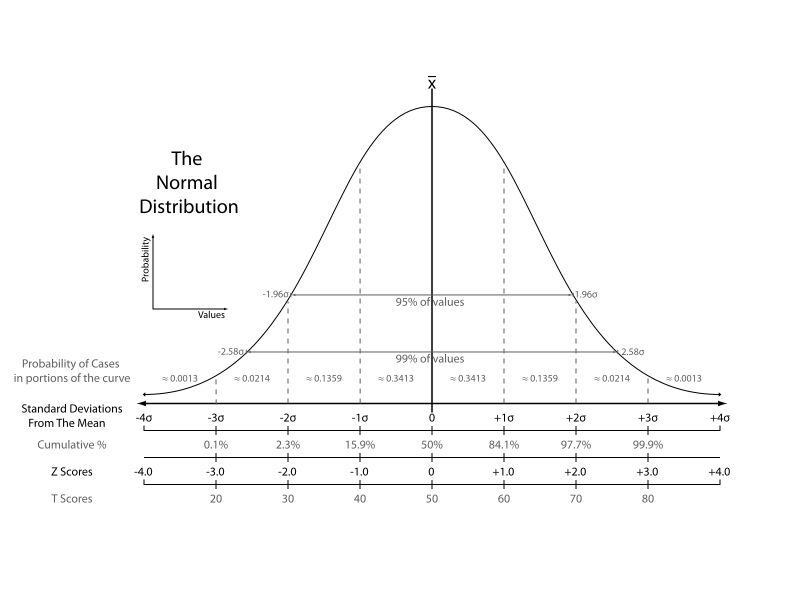
\includegraphics[width=0.6\linewidth]{picture/normal.png}
    \caption{Normal distribution.}
    \label{fig:normal distribution}
\end{figure}
We used the following test to identify nconsistent values in numerical columns like negative dates...
A normal distribution is a symmetric, continuous, and  bell-shaped distribution.
For Gaussian distributions, within one standard deviation from the mean lie 68\% of the values, while within 3 standard deviations lie 99.73\%, and within 6 standard deviations lie 99,99\% of the values (Figure~\ref{fig:normal distribution}).
Hence, we suppose that non-constant and non-discrete (non-clustering) numerical columns are Gaussian and identify extreme values as lying outside the sample mean plus/minus six sample standard deviations to cover 99.73\% of the distribution.
We denote this test by the extreme values test.
Although it successfully detects most of the extreme values within our data with a sufficiently small ratio of false negatives, it may give weird results if the distribution of the column is not Gaussian.
We recommend starting with a test of Gaussianity before proceeding with the extreme values test.
% subsection Extreme values (end)

\subsection{Completeness} % (fold)
\label{sub:Completeness}
The completeness of data is also an important concept to check. We construct an algorithm to flag rows with high ratio of missing values and we associate as error of type completeness error. This algorithm are present by the class method \texttt{check\_completeness} by the pseudo code \ref{completeness}.
% subsectionCompleteness (end)


\subsection{Accuracy} % (fold)
\label{sub:Accuracy }
\dhawat{TBC}
% subsectionAccuracy metric (end)
\subsection{Logical order relation} % (fold)
\label{sub:Logical order relation}
The idea behind this algorithm is to find ordering errors between two numerical columns by detecting if there is an inherent order between them and flagging the elements that does not respect it. For example all the values of the column \texttt{BIRTH\_YEAR} should be lower than there corresponding value in the column \texttt{DEATH\_YEAR} if not then it is an error. We proceed to a what we would call a tendency test between pairs of all numerical columns, let \texttt{column\_a} and \texttt{column\_b} be two numerical columns, we compute the ratio between the number of elements in \texttt{column\_a} that are lower to their corresponding value in \texttt{column\_b} (row-wise comparison) and the length of the columns. We start by dropping the missing values first to avoid any problems. if the ratio is high (let's say 99.99\% the threshold is a parameter that needs to be fixed to avoid too much false positives) that would mean that there is a hidden tendency between those two columns and that the values that does not respect that order might be outliers.
This algorithm is present in the class method \texttt{check\_tendency} and is presented in the pseudo code \ref{tendency}.
% subsection Logical order relation (end)

\subsection{Outlier detection with machine learning} % (fold)
\label{sub:Outlier detection with machine learning}
\begin{figure}[H]
    \centering
    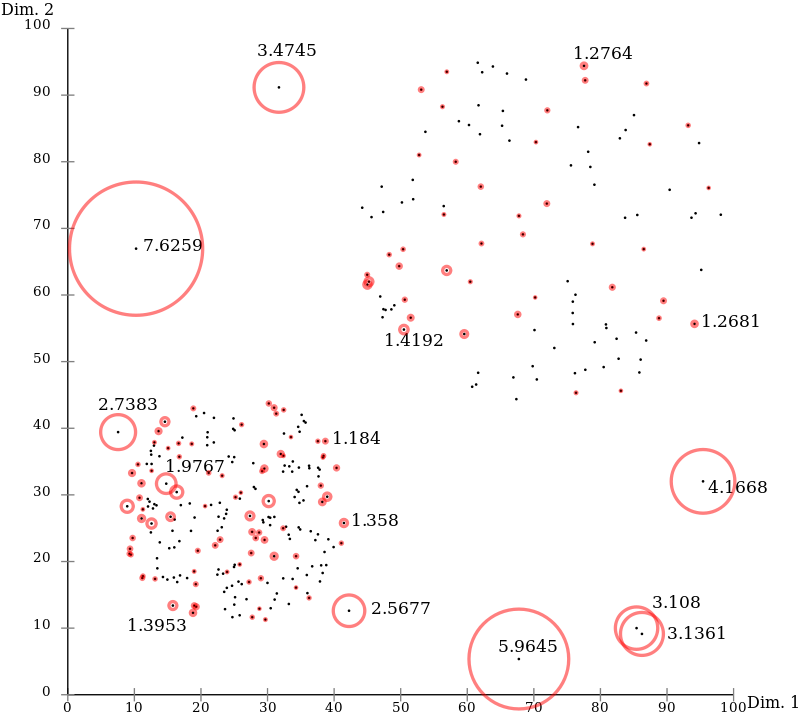
\includegraphics[width=0.6\linewidth]{picture/lof.png}
    \caption{Local Outlier Factor.}
    \label{fig:lof}
\end{figure}
The local outlier factor method, or LOF for short, is a technique that attempts to harness the idea of nearest neighbors for outlier detection.
It is an unsupervised machine learning anomaly detection method.
The local outlier factor is based on a concept of a local density, where locality is given by k nearest neighbors, whose distance is used to estimate the density.
By comparing the local density of an object to the local densities of its neighbors, one can identify regions of similar density, and points that have a substantially lower density than their neighbors. These are considered to be outliers.
The local density is estimated by the typical distance at which a point can be ``reached" from its neighbors.
The definition of ``reachability distance" used in LOF is an additional measure to produce more stable results within clusters.
Due to the local approach, LOF is able to identify outliers in a data set that would not be outliers in another area of the data set.
For example, a point at a ``small" distance to a very dense cluster is an outlier, while a point within a sparse cluster might exhibit similar distances to its neighbors.
The LOF test is available in our Python package by the class method \texttt{check\_outlier}.
This test is applied on the numerical columns gathered.
On tables containing \texttt{NaN} in numerical columns and since the LOF test does not apply to data containing missing values, we were facing the problem of dealing with the missing element before being able to to detect outliers by the LOF.
To overcome the problem of missing values data scientists use \textbf{imputation} methods.\\

\noindent
The imputation is process for fills missing data with synthetic values.
Imputation preserves all cases by replacing missing data with an estimated value based on other available information.
Once all missing values have been imputed, the data set can then be analysed using standard techniques for complete data.
There are different approach for imputing missing values \cite{corr_lede}:
\begin{enumerate}
    \item Deletion: removes all instances with missing values.
    \item Hot deck: missing data are filled with values from the same dataset.
    \item Imputation based on missing attributes: computes a new value from measures of central tendency as median, mode, mean,
          etc. The computed value is used for filling the missing data.
    \item Imputation based on non-missing attributes: a classification or regression model is built from available data to fill the missing values.
\end{enumerate}
Or for some table all rows contains missing values or most of them so the deletion option could not be used in the case were we are doing imputation over the hole table and not a specific columns.
From the last 3 methods we chose the imputation based on non-missing attributes using k-Nearest Neighbors provided by \href{https://scikit-learn.org/stable/modules/generated/sklearn.impute.KNNImputer.html}{sklearn}.
Missing values are imputed using the mean value from k-nearest neighbors found in the table. Two samples are close if the features that neither are missing is close.
% subsection  Outlier detection with machine learning (end)
\subsection{Frequency for logical errors} % (fold)
\label{sub:Frequency for logical errors}
As we already mentioned the step of detecting rows outlier of type logical error was done via the algorithm LOF preceded by an imputation method \ref{sub:Outlier detection with machine learning}.
Although finding the logical errors in a table (rows) is a difficult task in outlier detection, specifying their positions (rows, columns) is even harder.
Based on the idea that outliers occur less then inliers, we constructed an algorithm to detect logical error between couples of correlated rows in this way we specify directly the positions (rows, columns) of a part of the logical error and we overcome the difficulty of this task.
We introduce a pattern-based methods, which search for outlying/normal patterns and employ pattern frequency as a direct outlierness measure to detect outliers.
For sufficiently 2 correlated columns, the idea is to find for each element of the first column the associated elements from the second columns and find the frequency of the couple and flag couples with sufficiently low frequency.
\begin{figure}[H]
    \centering
    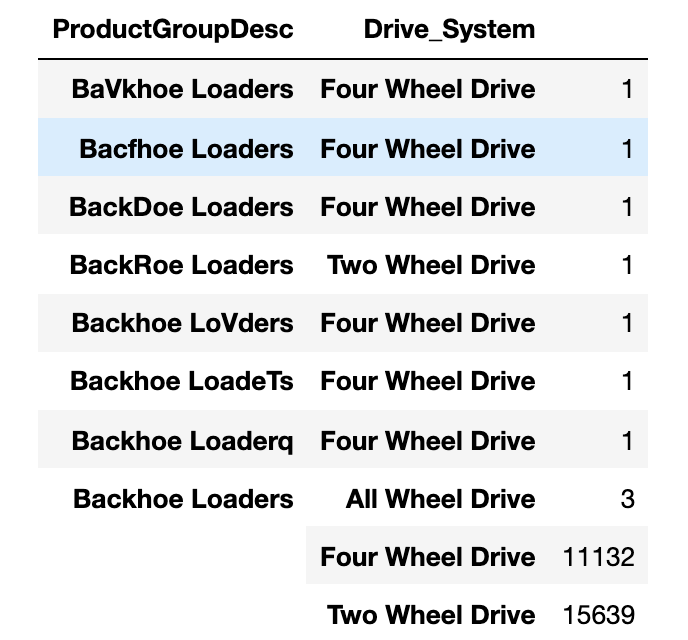
\includegraphics[width=0.6\linewidth]{picture/logic_err.png}
    \caption{Groups from 2 correlated columns.}
    \label{fig:logic_err}
\end{figure}
To simplify the idea we will consider an example from the table that we were provided. Figure \ref{fig:logic_err} represent the a sequences of couple of element from the columns \texttt{ProductGroupDesc} and \texttt{Drive\_system} and the frequency of occurences of each couple.
As we already mention the basic idea of outlier detection is that, in any table of data outlier occur less frequently then inlier.
By examining the frequencies of the the couple associated to \texttt{Backoe Loeders} we can deduce that \texttt{All Wheel Drive} occur clearly less then other frequencies and so it's an logical error. Moreover the high number of clusters in this column (11132, 15639) implies that all couples occurring 1 times are outliers, in this way we can also detect the spelling errors in the column \texttt{ProductGroupDesc} present in figure \ref{fig:logic_err} as the variant of \texttt{Backoe Loeders}
The same is applied for couple of categorical correlated
The test for detecting outlier of type logical error using the frequency is applied on couples of sufficiently correlated string columns, non unique, with categorical discrete aspect i.e. columns with clustering aspect.
As we already mentioned this algorithm we be held only on sufficiently correlated clustered columns, it is preceded by finding the matrix of correlations between sufficiently clustered categorical columns.
This algorithm is present in the class method \texttt{bad\_logical\_index} and as pseudo code in \ref{str_logic}.
% subsection Frequency for logical errors (end)

\subsection{Intra categorical extreme values} % (fold)
\label{sub:Intra categorical extreme values}
We proceed as in \ref{sub:Frequency for logical errors} applying a pattern-based method between categorical columns and numerical ones, to look for extreme values within a specific class of a category (\textit{e.g.} the distribution of the price of a specific class of the column \texttt{CAR}.). In order to do that we start by selecting categorical columns that contain very few classes (their ratio of uniqueness would be lower than a fixed threshold), for a categorical column and a given numerical column, we partition the values of the numerical column using the classes of the categorical one we get $m$ subsets, $m$ being the number of classes in the categorical column: $\{c_1: n_{1, c_1}, n_{2, c_1}, \ldots, n_{i, c_1}\}, \ldots, \{c_m: n_{j+1, c_m}, \ldots,  n_{l, c_m}\}$ with $c_1, \ldots, c_m$ the classes of the categorical column and $(n_i)_{i \leq l}$ the values of the numerical one. Then we proceed to an extreme value test on each subset.
It is very important to distinguish between the continuous numerical columns and the discrete ones because the testing procedure will not be the same, for the continuous numerical column we would use a \texttt{z-score} test and for the discrete ones we use the frequency of occurrences as in \ref{sub:Frequency for logical errors}.
This algorithm is present by the class method \texttt{check\_mixt\_logic} by the pseudo code \ref{mixed_logic}.
% subsection Intra categorical extreme values (end)

% section  Starategy used to detect bad data (end)

\section{Algorithm} % (fold)
\label{sec:Algorithm}
Different error types and data types force us to use different methods and algorithm to judge data quality. In light of this we decided to split our algorithm into several standalone module capable of being called independently of one another.
If the user wishes to simply use all the algorithm and with standard parameters we provided two methods for doing so. The first method is used to get rid of easier to detect errors such as duplicates and typos before (if wished) passing its results to the second method which will be a more in depth check. The first method is also fully identifiable as it is a major consideration for the company to be able to check afterward if the error is true and where it is.\\
On top of that we provided a class in which the user can load the data and pre-process it if needed. We wanted the code to be able to be used by someone with basic knowledge and have room if needed to fine tune each parameter independently if they have a deeper knowledge of the subject.\\
Let us then follow our outlined methods and inspect the first method algorithms and then the second method.


\subsection{First method}

\subsubsection{Typographical error algorithm}
\label{sub:Typographical error algorithm}
\begin{algorithm}[H]
    \SetKwData{Left}{left}\SetKwData{This}{this}\SetKwData{Up}{up}
    \SetKwFunction{Union}{Union}\SetKwFunction{FindCompress}{FindCompress}
    \SetKwInOut{Input}{input}\SetKwInOut{Output}{output}
    \Input{A column of a DataFrame, a minimum frequency threshold, A specified method to deal with clustering}
    \Output{Index of the DataFrame containing typographical errors}
    \BlankLine

    list\_incorrect$\leftarrow$ [~]\;
    words $\leftarrow$ get unique element from input column\;
    \If{method is affinity propagation}
    {
        lev\_similarity $\leftarrow$ \lForEach{element $w1$ in word, element $w2$ in word}{SequenceMatcher(w1, w2)}
        affprop $\leftarrow$ instance AffinityPropagation\;
        affprop\_label $\leftarrow$ affprop.fit(lev\_similarity).labels \;
        \eIf{affprop\_label is empty}
        {
            return list\_incorrect\;
        }
        {\For{cluster in affprop\_label}
            {list\_incorrect $\leftarrow$ list\_incorrect + incorrect\_grammar(column, cluster, threshold)\;}
        }
        return list\_incorrect
    }
    \Else{
        X $\leftarrow$ instance Vectorizer and transform words into it\;
        dict\_cluster $\leftarrow$ get clusters from MarkovClustering(X)\;
        \If{dict\_cluster is empty}
        {return list\_incorrect}
    }
    \caption{Typographical checking\label{typo}}
\end{algorithm}



\subsubsection{Duplicate errors algorithm}

\begin{algorithm}[H]
    \SetKwData{Left}{left}\SetKwData{This}{this}\SetKwData{Up}{up}
    \SetKwFunction{Union}{Union}\SetKwFunction{FindCompress}{FindCompress}
    \SetKwInOut{Input}{input}\SetKwInOut{Output}{output}
    \Input{A DataFrame}
    \Output{Index of the DataFrame duplicated, index of first duplicate}
    \BlankLine
    boolean\_idx $\leftarrow$ duplicated(dataframe, omit\_first)\;
    boolean\_first $\leftarrow$ duplicated(dataframe, all)\;

    index\_true $\leftarrow$ boolean\_idx(boolean\_idx) and boolean\_first(boolean\_first)\;

    return index(boolea\_idx == True), index\_true
    \caption{Duplication checking\label{duplicate}}
\end{algorithm}



\subsubsection{Extreme value algorithm}


\begin{algorithm}[H]
    \SetKwInOut{Input}{input}\SetKwInOut{Output}{output}
    \Input{A column of a DataFrame, a minimum frequency threshold, the uniqueness ratio of the column, a standard deviation multiplier, 2 uniqueness thresholds}
    \Output{Index of the DataFrame containing extreme values}
    \BlankLine

    \uIf{uniqueness $\geq$ threshold\_1 or uniqueness $\leq$ threshold\_2}{return [~] \;}
    \Else{
        mean $\leftarrow$ mean(column)\;
        std $\leftarrow$ std(column)\;

        upper\_bound $\leftarrow$ mean + threshold\_std * std\;
        lower\_bound $\leftarrow$ mean - threshold\_std * std\;

        idx $\leftarrow$ column where element is $\geq$ lower\_bound and $\leq$ upper\_bound\;
        return idx\;
    }
    \caption{Extreme value checking\label{extreme}}
\end{algorithm}



\subsubsection{Row completeness algorithm}
\begin{algorithm}[H]
    \SetKwInOut{Input}{input}\SetKwInOut{Output}{output}
    \Input{A DataFrame, a minimum threshold of empty values for rows, a minimum threshold of empty values for rows when low information columns are removed, a minimum threshold of empty values for columns}
    \Output{Index of the DataFrame containing rows with low completeness}
    \BlankLine
    mean\_none\_row1 $\leftarrow$ mean(NA in dataframe.rows)\;
    index\_1 $\leftarrow$ index(rows $\geq$ thresh\_row\_1 NA)\;
    \BlankLine
    mean\_none\_col $\leftarrow$ mean(NA in dataframe.columns)\;
    index\_col $\leftarrow$ index(columns $\geq$ thresh\_col NA)\;
    \BlankLine
    \For{idx in index\_col}{drop column[idx] of dataframe}
    \BlankLine
    mean\_none\_row2 $\leftarrow$ mean(NA in dataframe.rows)\;
    index\_2 $\leftarrow$ index(rows $\geq$ thresh\_row\_2 NA)\;
    \BlankLine
    idx = index\_1 and index\_2\;
    return idx
    \caption{Row completeness checking\label{completeness}}
\end{algorithm}



\subsubsection{Tendency algorithm}
\begin{algorithm}[H]
    \SetKwInOut{Input}{input}\SetKwInOut{Output}{output}
    \Input{A DataFrame, a minimum threshold for an observed order between variable to become a rule to discriminate outliers upon.}
    \Output{Index and column of the DataFrame containing rows which breaks the tendency}
    \BlankLine

    dict\_tendency $\leftarrow$ \{\}\;

    \For{column1 in numerical\_columns(dataframe)}{
        \For{column2 in numerical\_columns(dataframe)}{
            dataframe $\leftarrow$ drop(dataframe(column1, column2), any rows with NA)\;
            tendency $\leftarrow$ $\frac{size(dataframe(column1) \leq dataframe(column2))}{size(dataframe)}$\;
            \BlankLine
            \If{tendency $\geq$ tendency\_threshold}{
                \If{size(dataframe(column1) $\geq$ dataframe(column2)) $\geq$ 1}{
                    dict\_tendency[(column1, column2)] $\leftarrow$ index(dataframe(column1) $\geq$ dataframe(column2))\;
                }
            }
        }
    }
    return dict\_tendency
    \caption{Tendency checking\label{tendency}}
\end{algorithm}

\subsection{Second method} % (fold)
\label{sub:Second method}

% subsectionSecond method (end)

\subsubsection{Whole row outlier detection algorithm}
\begin{algorithm}[H]
    \SetKwInOut{Input}{input}\SetKwInOut{Output}{output}
    \Input{A DataFrame}
    \Output{Index of the DataFrame containing rows which are deemed to be outliers using the lof method}
    \BlankLine

    \If{dataframe has NA}{
        dataframe $\leftarrow$ KNNImputer(dataframe)\;
    }
    \BlankLine
    clf $\leftarrow$ instancize LocalOutlierFactor\;
    prediction $\leftarrow$ clf.fit\_predict(dataframe)\;
    idx $\leftarrow$ index(prediction == outlier)\;
    \BlankLine
    return idx
    \caption{Whole row outlier checking\label{outlier}}
\end{algorithm}

\subsubsection{Text categorical logic algorithm}
\label{Text categorical logic algorithm}
\begin{algorithm}[H]
    \SetKwInOut{Input}{input}\SetKwInOut{Output}{output}
    \Input{A DataFrame, a threshold for of the uniqueness for columns, a threshold for the number of time a categorical error happens}
    \Output{Index of the DataFrame and two columns in which a categorical error is made}
    \BlankLine

    dataframe $\leftarrow$ dataframe(index not rejected by first method)\;

    col\_names $\leftarrow$ [~]\;
    idxes $\leftarrow$ [~]\;
    \For{column1 in verbal\_column(dataframe)}{
        \For{column2 in verbal\_correlated\_columns(dataframe, column1)}{
            \If{column1 not == column2 and uniqueness(column1) $\leq$ thres\_uniqueness and uniqueness(column2) $\leq$ thres\_uniqueness}{
                occurences $\leftarrow$ get\_contingency\_table(dataframe(column1), dataframe(column2))\;
                elements $\leftarrow$ dataframe((column1, column2) not NA)\;
                \For{elem in unique(elements(column1))}{
                    \For{(e, value) in (occurences(elem), index(occurences(elem))}{
                        \If{e $\leq$ thres\_error}{
                            idxes $\leftarrow$ idxes $+$ elements(column2 where index = elements(column2) == value and elements(column1) == elem)\;
                            col\_names $\leftarrow$ col\_names $+$ (column1, column2)
                        }
                    }
                }
            }
        }
    }

    return idxes, col\_names
    \caption{Text categorical logic error checking\label{str_logic}}
\end{algorithm}




\subsubsection{Mixed number text categorical logic algorithm}

\begin{algorithm}[H]
    \SetKwInOut{Input}{input}\SetKwInOut{Output}{output}
    \Input{A DataFrame, a threshold for of the uniqueness for verbal columns, a threshold for numerical columns, a standard deviation multiplier}
    \Output{Index of the DataFrame and two columns in which a categorical error is made}
    \BlankLine

    dataframe $\leftarrow$ dataframe(index not rejected by first method)\;

    col\_names $\leftarrow$ [~]\;
    idxes $\leftarrow$ [~]\;
    list\_seen $\leftarrow$ [~]\;

    \For{column1 in verba\_columns(dataframe)}{
        \If{uniqueness(column1) $\leq$ threshold\_verbal}{
            \For{column2 in numerica\_columns(dataframe)}{
                \If{(column1, column2) not in list\_seen and uniqueness(column2) $\geq$ thresol\_numerical}{
                    elements $\leftarrow$ dataframe((column1, column2) not NA)\;
                    \For{elem in unique(elements(column1))}{
                        array\_values $\leftarrow$ elements(column2 where elements(column1) == elem)\;
                        \If{array\_values not empty}{
                            index\_outliers $\leftarrow$ Algorithm\_2(array\_values, 0.1, thresh\_std)\;
                            \If{index\_outliers not empty}{
                                value\_outliers $\leftarrow$ array\_values(index\_outliers)\;
                                idxes $\leftarrow$ idxes $+$ index(element(column2 where element(column2) == value\_outliers))\;
                                col\_names $\leftarrow$ col\_names $+$ (column1, column2)\;
                            }
                        }
                    }
                    list\_seen $\leftarrow$ list\_seen + (column1, column2)
                }
            }
        }
    }

    return idxes, col\_names

    \caption{Mixed number text categorical logic error checking\label{mixed_logic}}
\end{algorithm}


% sectionAlgorithm (end)

\section{Experiments} % (fold)
\label{sec:Experiments}

At the start of the challenge our correspondant at Foyer shared with us a dataset comprised of 100000 columns and 54 columns. This dataset represented a real life example of sales of agricultural machinery. The types of column that we had were composed of numerical quantitative columns e.g. price, numerical category  e.g. Model Id but also verbal columns such as the state in which the sale took place.
Not all the columns were in a type directly usable such as \texttt{saledate} which were in a non classical format. \\

In this section we will discuss the type of errors caught by our algorithms, their strengths and shortcomings.
In the first method we used \ref{duplicate} for finding duplicate, this method returns both the 'true' index and one of the duplicated index for comparison.
\subsection{First method}

\begin{figure}[H]
    \centering
    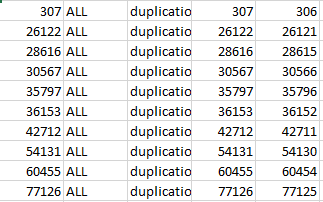
\includegraphics[scale=0.8]{picture/exp_duplicated.png}
    \label{fig:exp_duplicate}
    \caption{Extract from the returned table of error featuring duplication errors.}
\end{figure}

As we can see in the first line we do have a duplication in index 307 and 306 which indeed represent a duplicate in the original data. If we look at the origin data we get \ref{fig:exp_duplicate_db}. In terms of speed of execution is it both scalable and accurate, in the order of a second for 5 millions entries.

\begin{figure}[h]
    \centering
    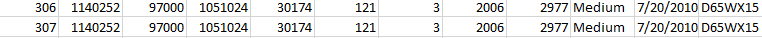
\includegraphics[width=\linewidth]{picture/exp_duplicated_db.png}
    \label{fig:exp_duplicate_db}
    \caption{Extract from the original dataset, here only a few column were taken for tidiness's sake.}
\end{figure}

The algorithm used for finding typographical errors \ref{typo} can be illustrated using the same method.

\begin{figure}[h]
    \centering
    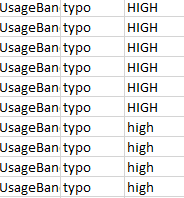
\includegraphics[scale=0.8]{picture/exp_typo.png}
    \label{fig:exp_typo}
    \caption{Extract from the returned table of error featuring typographical errors.}
\end{figure}
The figure \ref{fig:exp_typo} shows that in the column 'UsageBand' multiple instances of the values 'HIGH' and 'high' were detected as errors. Indeed after confirmation with our correspondant it is an induced error. The correct spelling is 'High', both with the affinity propagation and markov clustering we get this types of results. However, when the database gets bigger and more words starts to appear in a cluster, the base affinity propagation clustering fails to scale up both in terms of speed and performance because of the weak pairwise metric associated to the affinity propagation algorithm. The markov chain clustering methods on the other hand can be used even in high columns or row counts while still being tractable but give less desirable results in lower column counts. \\

For correcting numerical values while still being able to clearly tell in which column the error is we used the \ref{extreme} algorithm.

\begin{figure}[h]
    \centering
    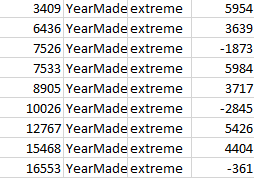
\includegraphics[scale=0.8]{picture/exp_extreme.png}
    \label{fig:exp_extreme}
    \caption{Extract from the returned table of error featuring extreme values errors.}
\end{figure}

On numerical column it flags as outliers extreme values using a z\_score method. On columns such as \texttt{YearMade} (of the machinery) it correctly flags absurd years such as negative years and far into the future years. Being a methods which flags when the value is well outside the mean it sometimes fails when considering columns which are made up of a continuous variable such as \texttt{SalePrice} but who has a latent variable such as \texttt{ModelId}. \\ Another type of column which might be a problem with \ref{extreme} is when the data is numerical but purely qualitative such as \texttt{datasource}. It is comprised of numbers but only two of them representing which office aggregated the data. For this type of error we implemented a check inside \ref{extreme} to abort if the ratio of uniqueness of the column is too low.\\
As for the speed and scalability of the method, on nearly 900000 cells it was in the order of a few seconds. On a larger dataset tested in collaboration of foyer it was similarly fast.

For the algorithm \ref{completeness} we can check \ref{fig:exp_completeness}, that it shows multiple exact same track type tractor-dozer down to the model id having on this subset of column less information.

\begin{figure}[h]
    \centering
    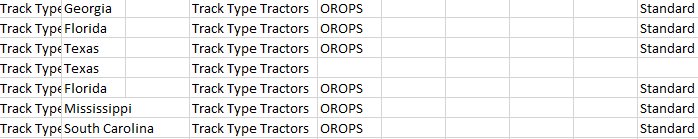
\includegraphics[width=\linewidth]{picture/exp_completeness_db.png}
    \label{fig:exp_completeness}
    \caption{Extract from the returned table of error featuring low row completeness errors.}
\end{figure}
On the other column there is also less information. Is is not stricto sensu an error but in our view it doesn't bring enough information to be useful.

\subsection{Second method}
A general trend for the second method algorithm is that they give harder to interpret results. Not all because of inability to target individual error cells but because trey rely on covariance and tendency between columns and as such need a deeper knowledge of the subject at hand to check if the reported error is indeed a true one.

The algorithm \ref{tendency} only operates on columns which are numerical in nature. A working example might be as shown in \ref{fig:exp_tendency} where we check \texttt{YearMade} against \texttt{saledate}. Up to at least 99,9\% in this case the order is preserved and is recognized by our algorithm. It sometimes fails in assessing the order due to the presence of lot's of outliers.
\begin{figure}[h]
    \centering
    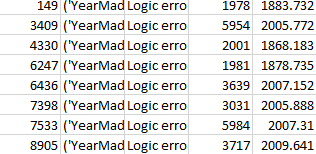
\includegraphics[scale=0.8]{picture/exp_tendency.png}
    \label{fig:exp_tendency}
    \caption{Extract from the returned table of error featuring tendency order errors.}
\end{figure}

In the algorithm \ref{outlier} we get to use the collective result of our previous methods to filter the flagged index. We leverage this to create a temporary higher data quality dataset which allows us to impute which otherwise would results in a low count of possible neighbors. In our case it appears to be (at least on the training set) an low risk low reward method, only flagging 10's indices in place of potentially hundreds for other methods. It however has a severe drawback that the imputation doesn't scale up with the number of rows very well. This methods can take up to a few minutes for a 900 000 data points.\\


One of the most interesting algorithm for us was the str and mixed type logic detector. To validate this kind of error we had to check the frequency and the validity of certain association between categories.
Typically if a certain type of agricultural machinery registered as a wheel loader but doesn't have the proper drive system it is usually a low frequency type of event and thus is detected by \ref{str_logic}.
Low frequency event, or for numerical table aberrant values can be detected using the mixed type logic algorithm \ref{mixed_logic}. For the verbal algorithm since it precomputes the correlation matrix it can be quite fast at low cells counts but costly if working on a billion data point. Even though the mixed type doesn't use this correlation matrix it can still be slow at similar numbers of inputs.
As we will discuss in the next section optimisation and adaptations can be improved upon.
% sectionExperiments (end)

\section{Discussions} % (fold)
\label{sec:Discussions}
We tested the algorithm on a data set provided by Foyer, after comparing the flagged errors with the known errors injected by the company, it showed a success rate of 36\%, we made the choice of using very strict thresholds to avoid false positives to not flood the user with information, the major positive component is the fact that the algorithm runs relatively fast. We also proceeded to a quick test on one of the data sets of the company and the test were very encouraging as well. \
The next step would be to control the number of false positives that we get, one way to proceed would be to improve the choice of the thresholds, also for the \texttt{check\_mixt\_logic()} to run a correlation test between columns in order to only consider the columns that are sufficiently correlated.
in addition regarding the typo algorithm, we observed that if we run the Affinity Propagation algorithm twice, the first time on the whole data set of words and the second time on the proposed clusters, it highly improves the results and we end up getting a better clustering of the words, which makes it easier to detect spelling errors and suggest a correction to the user. \
Another axis of research, that we did not have time to explore is about the classification of the missing values (nan's) in the data set, we wanted to implement a solution that would help sort between the null value  missing completely at random, missing at random and missing not at random, which is an outlier types of missing values. Detecting which kind of missing value is important in the imputation phase of pre-processing the data.
% section Discussions (end)

\section*{Acknowledgments} % (fold)
\label{sec:Acknowledgments}
We would like to thank AMIES for this beautiful opportunity and Foyer for providing us with the technical support and supervising (special thanks to Alexandre Hotton).


% sectionAcknowledgments (end)

\begin{thebibliography}{999}

    \bibitem{pan_cos_chen}
    Guansong Pang, Longbing Cao and Ling Chen:
    \emph{Outlier Detection in Complex Categorical Data
        by Modelling the Feature Value Couplings.}

    \bibitem{amazon}
    Sebastian Schelter, Dustin Lange, Philipp Schmidt, Meltem Celikel, Felix Biessmann
    \emph{Automating Large-Scale Data Quality Verification}

    \bibitem{dai_yosh_pars}
    Wei Dai, Kenji Yoshigoe and William Parsley
    \emph{Improving Data Quality Through Deep Learning and Statistical Models}

    \bibitem{corr_lede}
    David Camilo Corrales, Agapito Ledezma and Juan Carlos Corrales
    \emph{From Theory to Practice: A Data Quality Framework
        for Classification Tasks}

    \bibitem{Hawking}
    Simon Hawkins, Hongxing He, Graham Williams, Rohan Baxte:
    \emph{Outlier Detection Using Replicator Neural Networks}

\end{thebibliography}
\end{document}
